

\subsection{Fast multipole method for the {\gpu}}

We will now concentrate on the algorithmic redesign of the {\fmm} for {\gpu} computing, whereas a more in-depth discussion of the implementation details takes place in \S\ref{implementation}. As such, we start by noticing that the most time-consuming stages of the {\fmm} algorithm are: the near-field calculations, and the downward sweep. As we observed in \S\ref{subsec:fmm_back}, these stages can take  of the runtime in a serial implementation of the algorithm, and continue to dominate in parallel implementations despite parallel overheads.


Let us discuss in more detail the computations performed by these two stages.  In the case of the near-field calculations, the problem is to compute the mutual interactions of particles in many small- to medium-size domains, with each domain containing at most a few hundred particles. Therefore, the near-field calculation problem can be reduced to efficiently implementing the direct particle interactions for each domain, and as such, this is a special case of the -body problem, where interactions are computed only with a subset of the  particles. Furthermore, the near-field calculation retains the distinctive features of being computationally intensive and highly parallel. Therefore, this problem can be efficiently mapped to the \gpu\ architecture, achieving high performance, as reported in~\cite{NylandHarrisPrins2007,BellemanEtal2008}.
We note that, as pointed out by \cite{NylandHarrisPrins2007}, a balanced \fmm\ execution in the \gpu\ will perform the near-field direct evaluation with a larger set of particles per box than in the {\cpu} case. This difference is due to the higher efficiency achieved by the {\gpu} in the near-field calculations, as compared to the far-field calculations. Consequently, the optimal workload distribution between these two stages is different in the {\gpu} and {\cpu} executions.

In the downward sweep, the computations are dominated by the transformation of multipole expansions into local expansions ({\ML} step). Tens of thousands of concurrent {\ML} transformations are computed in the {\fmm} algorithm, this being the reason for such a high computational intensity. Each of these transformations can be expressed in the form of a matrix-vector multiplication, where each matrix is dense, of size (), where  corresponds to the number of terms of a truncated {\ME}. 
The algorithmic steps of the downward sweep are: 
\begin{enumerate}
\item For every node of the hierarchical tree, we obtain the list of clusters that belong to the same level, effectively computing the interaction list of each node. 
\item Then for every node (or evaluation cluster) in the tree, the multipole expansions of each cluster in its interaction list are transformed into a local expansion centered at the evaluation cluster.
\item Finally, the cluster's local expansion is obtained by aggregating the local expansions obtained from the {\ML} transformation of all the clusters in the interaction list, this step is referred to as the \emph{reduction}.
\end{enumerate}

We present the following example to illustrate the parallelism and computational intensity of the downward sweep stage. Consider a two-dimensional case () where the computational domain is hierarchically decomposed by a uniform tree (a quadtree) with  levels of spatial refinement. Such a tree will approximately have  nodes, where each node will transform on average  multipole expansions (more precisely, this number corresponds to the size of the node's interaction list). Therefore, the approximate number of {\ML} transformations computed are . For deeper trees, more transformations would be needed. 

In the original algorithm for the {\ML} transformation, the multipole expansion of a given cluster , with center  and multipole coefficients , is transformed into a local expansion for cluster  with center at . The result of the transformation will give the local expansion coefficients . In the -dimensional case, both the coordinates and expansion terms are usually represented by complex numbers. The {\ML} transformation in its matrix-vector multiplication form has a transformation matrix , with  complex elements, . These elements can be obtained using the following expression:
 

As previously noted, the {\ML} stage is highly parallel and computationally intensive. However, in order to obtain a high-performance implementation for the {\gpu}, the {\ML} stage needs to be reformulated.

\subsubsection{Reformulation of the {\ML} problem}

As a first approach,  one can consider distributing the mat-vec operations across threads.  That is, each {\cuda}-thread would perform one such operation.  Suppose that the evaluation requires a truncation parameter , as required for high-accuracy simulations; see for example \cite{CruzBarba2009}. In that case, each matrix has a size of , requiring 2304 bytes of storage.  Thus, in the {\gpu} shared memory of 16~kB one could fit a maximum of  such matrices, which implies that a maximum of  threads could be run in one multi-processor at a time. Clearly this number of threads is much too small\,---as discussed in \S\ref{hardware}, more than one hundred threads per {\sm} are needed in order to hide memory transfer latencies. Alternatively to storing the transformation matrix in shared memory, it is feasible to use Equation \eqref{eq:M2Lmat} to compute the matrix elements as the matrix-vector multiplication takes place (also known as matrix-free format). 
\begin{figure}
	\centering
	\subfigure[Traversing the matrix diagonals.]
		{\label{fig:m2la}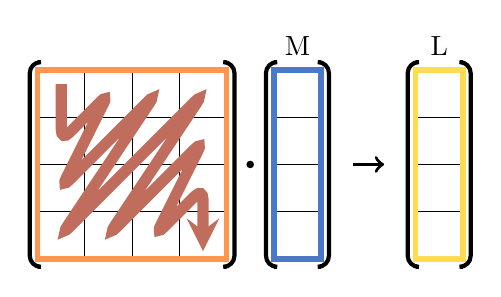
\begin{tikzpicture}

\definecolor{meColor}{rgb}{0.29, 0.48, 0.78}
\definecolor{leColor}{rgb}{1.0,0.86,0.31}
\definecolor{m2lColor}{rgb}{1.0,0.59,0.31}
\definecolor{threadColor}{rgb}{0.65,0.18,0.10}

\begin{scope}[scale=0.40]
\draw (3,6.75) node {};
    \draw (8.25,6.75) node {M};
    \draw (12.75,6.75) node {L};
\draw[step=1.5,black] (0,0) grid (6,6); \draw[step=1.5,black] (7.5,0) grid (9,6); \draw[step=1.5,black] (12,0) grid (13.5,6); \draw[m2lColor, line width=2pt] (0,0) rectangle (6,6); \draw[meColor, line width=2pt] (7.5,0) rectangle  (9,6); \draw[->,black, very thick] (10,3) -- (11,3);
    \draw[leColor, line width=2pt] (12,0) rectangle (13.5,6); \fill[black] (6.75,3) circle (0.12); \draw[black, line width=1.5pt, rounded corners]  (0, 6.25) -- ++(-0.25,0)  -- ++(0,-6.5) -- ++(0.25,0); \draw[black, line width=1.5pt, rounded corners]  (6, 6.25) -- ++(0.25,0)  -- ++(0,-6.5) -- ++(-0.25,0); \draw[black, line width=1.5pt, rounded corners]  (7.5, 6.25) -- ++(-0.25,0)  -- ++(0,-6.5) -- ++(0.25,0); \draw[black, line width=1.5pt, rounded corners]  (9, 6.25) -- ++(0.25,0)  -- ++(0,-6.5) -- ++(-0.25,0); \draw[black, line width=1.5pt, rounded corners]  (12, 6.25) -- ++(-0.25,0)  -- ++(0,-6.5) -- ++(0.25,0); \draw[black, line width=1.5pt, rounded corners]  (13.5, 6.25) -- ++(0.25,0)  -- ++(0,-6.5) -- ++(-0.25,0); \draw[>=stealth,->, threadColor!70, solid, line width=4pt] {[rounded corners] 
          (0.75, 5.55) -- (0.75, 3.75)
      -- (2.25, 5.25) -- (0.75, 2.25)
      -- (3.75, 5.25) -- (0.75, 0.75)
      -- (5.25, 5.25) -- (2.25, 0.75)
      -- (5.25, 3.75) -- (3.75, 0.75)
      -- (5.25, 2.25) -- (5.25, 0.25)};
\draw (0.75, 0.75) node{};\draw (2.25, 0.75) node{};
    \draw (3.75, 0.75) node{};
    \draw (5.25, 0.75) node{};
    \draw (0.75, 2.25) node{};\draw (2.25, 2.25) node{};
    \draw (3.75, 2.25) node{};
    \draw (5.25, 2.25) node{};
    \draw (0.75, 3.75) node{};\draw (2.25, 3.75) node{};
    \draw (3.75, 3.75) node{};
    \draw (5.25, 3.75) node{};
    \draw (0.75, 5.25) node{};\draw (2.25, 5.25) node{};
    \draw (3.75, 5.25) node{};
    \draw (5.25, 5.25) node{};
\draw (8.25, 5.25) node{};\draw (8.25, 3.75) node{};
    \draw (8.25, 2.25) node{};
    \draw (8.25, 0.75) node{};
\draw (12.75, 5.25) node{};\draw (12.75, 3.75) node{};
    \draw (12.75, 2.25) node{};
    \draw (12.75, 0.75) node{};
\end{scope}
\end{tikzpicture} }
	\subfigure[By rows.]
		{\label{fig:m2lb}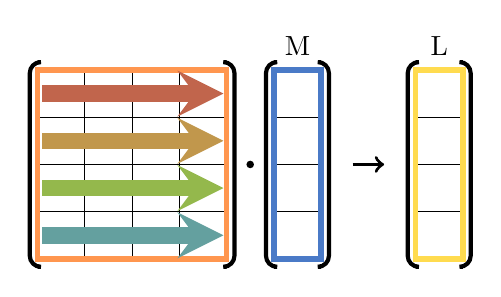
\begin{tikzpicture}

\definecolor{meColor}{rgb}{0.29, 0.48, 0.78}
\definecolor{leColor}{rgb}{1.0,0.86,0.31}
\definecolor{m2lColor}{rgb}{1.0,0.59,0.31}
\definecolor{thread0Color}{rgb}{0.65,0.14,0.00}
\definecolor{thread1Color}{rgb}{0.65,0.42,0.00}
\definecolor{thread2Color}{rgb}{0.40,0.60,0.00}
\definecolor{thread3Color}{rgb}{0.13,0.47,0.46}

\begin{scope}[scale=0.40]
\draw (3,6.75) node {};
    \draw (8.25,6.75) node {M};
    \draw (12.75,6.75) node {L};
\draw[step=1.5,black] (0,0) grid (6,6); \draw[step=1.5,black] (7.5,0) grid (9,6); \draw[step=1.5,black] (12,0) grid (13.5,6); \draw[m2lColor, line width=2pt] (0,0) rectangle (6,6); \draw[meColor, line width=2pt] (7.5,0) rectangle  (9,6); \draw[->,black, very thick] (10,3) -- (11,3);
    \draw[leColor, line width=2pt] (12,0) rectangle (13.5,6); \fill[black] (6.75,3) circle (0.12); \draw[black, line width=1.5pt, rounded corners]  (0, 6.25) -- ++(-0.25,0)  -- ++(0,-6.5) -- ++(0.25,0); \draw[black, line width=1.5pt, rounded corners]  (6, 6.25) -- ++(0.25,0)  -- ++(0,-6.5) -- ++(-0.25,0); \draw[black, line width=1.5pt, rounded corners]  (7.5, 6.25) -- ++(-0.25,0)  -- ++(0,-6.5) -- ++(0.25,0); \draw[black, line width=1.5pt, rounded corners]  (9, 6.25) -- ++(0.25,0)  -- ++(0,-6.5) -- ++(-0.25,0); \draw[black, line width=1.5pt, rounded corners]  (12, 6.25) -- ++(-0.25,0)  -- ++(0,-6.5) -- ++(0.25,0); \draw[black, line width=1.5pt, rounded corners]  (13.5, 6.25) -- ++(0.25,0)  -- ++(0,-6.5) -- ++(-0.25,0); \draw[>=stealth,->, thread0Color!70, solid, line width=6pt] (0.15, 5.25) -- (5.90, 5.25); \draw[>=stealth,->, thread1Color!70, solid, line width=6pt] (0.15, 3.75) -- (5.90, 3.75); \draw[>=stealth,->, thread2Color!70, solid, line width=6pt] (0.15, 2.25) -- (5.90, 2.25); \draw[>=stealth,->, thread3Color!70, solid, line width=6pt] (0.15, 0.75) -- (5.90, 0.75); \draw (0.75, 0.75) node{};\draw (2.25, 0.75) node{};
    \draw (3.75, 0.75) node{};
    \draw (5.25, 0.75) node{};
    \draw (0.75, 2.25) node{};\draw (2.25, 2.25) node{};
    \draw (3.75, 2.25) node{};
    \draw (5.25, 2.25) node{};
    \draw (0.75, 3.75) node{};\draw (2.25, 3.75) node{};
    \draw (3.75, 3.75) node{};
    \draw (5.25, 3.75) node{};
    \draw (0.75, 5.25) node{};\draw (2.25, 5.25) node{};
    \draw (3.75, 5.25) node{};
    \draw (5.25, 5.25) node{};
\draw (8.25, 5.25) node{};\draw (8.25, 3.75) node{};
    \draw (8.25, 2.25) node{};
    \draw (8.25, 0.75) node{};
\draw (12.75, 5.25) node{};\draw (12.75, 3.75) node{};
    \draw (12.75, 2.25) node{};
    \draw (12.75, 0.75) node{};
\end{scope}
\end{tikzpicture} }
	\caption{Sketch of different strategies for \ML\ computation.}
	\label{fig:M2Lversions}
\end{figure}   

When performing the matrix-vector product in matrix-free format, one can ``traverse'' the matrix such that the matrix terms are efficiently calculated by reusing the computations performed to obtain the previous terms. Therefore, one can reuse a part of both the binomial and the power terms by traversing the diagonals of the matrix, as sketched in Figure \ref{fig:m2la}.  This represents a strategy for matrix creation and multiplication that is efficient from the point of view of operations that it performs, in both the {\gpu} and {\cpu} architectures.  Moreover, for the {\gpu}, by assigning the computations of one matrix-vector multiplication to only one {\cuda}-thread, thread synchronization is not required. Consider now that each thread block performs the transformations of only one {\ME} for all the interaction list, accounting for an estimated  {\ML} transformations. During computation, the results of the transformation are stored in shared memory. With a maximum  of  concurrent thread blocks per multi-processor in the GT200 \gpu, we have a maximum of  active threads running on the multiprocessor.  This \NV\ {\gpu} allows a maximum of 512 threads in each thread block and 1024 active threads per {\sm}~\cite[][p.\,8]{cuda-guide}, and thus the approach just described could achieve less than one third of the maximum thread capacity of each {\sm}, without considering the register usage per thread. 
When the translation of an {\ME} is finished, one needs to move the result from shared memory to global memory, in the form of one {\LE} consisting of  floats. Hence, transforming one {\ME} for all the interaction list results in the movement of  floats. 
For instance, translating one {\ME} of  results in 648 floats that need to be stored in global memory, which at the hardware level results in  a minimum of twenty 128-byte and one 32-byte memory transactions (see \S\ref{subsec:mem_management} for a more complete discussion on memory management). When transferring the results to global memory, the memory transactions are executed by the thread-block one after the other, resulting in a stage where only memory transactions take place. A considerable disadvantage of such a memory-intensive stage is that multithreading is less effective in hiding the  memory latency when the number of active threads is small. 
Nevertheless, our implementation using this approach sustained 20 Gop/s and was able to perform  million translations per second, using a single C1060 {\tesla} card. 

\medskip

\begin{figure*}\begin{center}
	\begin{lstlisting}
	int k = 12;
	int n = threadIdx.x;
	    
	float ac, bd;
	tkn1_r = t_r;
	tkn1_i = t_i;
	    
	for (m = 1; m < k+n+1; m++)  // tkn1 = tkn1 * t
	{
	    ac      = tkn1_r;
	    bd      = tkn1_i;
	    tkn1_r = ac * t_r - bd * t_i;
	    tkn1_i = ac * t_i + bd * t_r;
	}

	\end{lstlisting}
\caption{Code snippet for computing the complex power , with . This code shows a for-loop with a variable number of iterations.}
\label{code:loop_divergence}
\end{center}
\end{figure*}


\begin{figure*}\begin{center}
	\begin{lstlisting}
	#define P 12
	
	int m;
	float ac, bd;
	float tn1_r = t_r;
	float tn1_i = t_i;
	
	#pragma unroll
	for (int m = 1; m < P; m++)
	{
	    if (threadIdx.x >= m) // tn1 = tn1 * t
	    {
	        ac   = tn1_r;
	        bd   = tn1_i;
	        tn1_r = ac * t_r - bd * t_i;
	        tn1_i = ac * t_i + bd * t_r;
	    }
	}

	\end{lstlisting}
\caption{Code snippet for computing the complex power , with . This code shows a for-loop where the number of iteration has been fixed at compile time to , and it uses a conditional for computing only the relevant power to each thread.}
\label{code:loop_known_num_iter}
\end{center}
\end{figure*}

The performance of the implementation just described is very much below the theoretical peak for both throughput and bandwidth of a C1060 {\tesla} card. An assessment of the {\cuda} kernel implementation revealed that its main limitation was the inefficiency of the memory transfers to and from global memory. This was due to two problems: first, many of the memory transfers were non-coalesced (i.e. adjacent threads reading adjacent memory values, see \S\ref{subsec:mem_management} for a full explanation), thus the \emph{effective bandwidth} used by the kernel was very low when compared against the theoretical performance of the card; and second, the kernel did not have enough active threads working per {\sm} to effectively hide the latency of the memory transfers, making the efficiency of the kernel implementation suffer. These two problems can be tracked down to a flaw in the design of our algorithm: using only one {\cuda} thread to perform a single translation.
The resulting kernel was resource-intensive since the diagonally traversing matrix-free multiplication required too many variables to store the state of the computations and to control the flow of the program, thus limiting the total number of active threads per {\sm}.
Additionally, having only one thread to perform each translation made it difficult to use multiple threads to perform collaborative memory transactions. 

Desirable features of a more optimized kernel would be for it to be: (\emph{i}) \emph{simpler}, requiring less variables to store the state of its execution, thus allowing more threads to be active at a time; (\emph{ii}) \emph{more parallel}, allowing the use of more concurrent threads, and to use coordinated collaboration between threads for performing memory transfers. 

Now, let us examine again Equation~\eqref{eq:M2Lmat}. A more parallel alternative to traverse the matrix is to have multiple {\cuda} threads assigned to traversing different rows of the matrix, as each row can be computed concurrently with each other; see Figure~\ref{fig:m2lb}.
As with the diagonal-traversal but to a more moderate extent, the row-traversal can also be implemented so that it reuses a part of both the binomial and the power terms.

Let us consider for a moment a straightforward implementation to obtain the powers in Equation \eqref{eq:M2Lmat} shown in the code fragment in Figure~\ref{code:loop_divergence}. What characterizes this simple approach is that the number of iterations per thread will depend on , which takes a different value for every thread. This straightforward implementation would have two problems: first, threads within a thread-block naturally stop at different points provoking the threads within a warp to diverge; second, loop unrolling would be unavailable as the compiler can only effectively unroll loops with known trip counts.

In our implementation, we separated the computation of powers in Equation \eqref{eq:M2Lmat} into two steps in order to minimize thread divergence, and to use compiler optimizations such as loop unrolling. In the first step of the calculation, the term  is computed by each thread; and in the second step, the next    factors, common to all threads, are multiplied. When computing the first step, we use a for-loop but with a fixed number of iterations (, with  the variable containing the truncation level of the {\ME}) and an \emph{if} conditional for computing only up to the power relevant to the thread; see the code fragment in Figure~\ref{code:loop_known_num_iter}. This approach minimizes thread divergence at the cost of a small overhead of evaluating a few extra empty iterations. However, the overhead is minimal when compared to the performance that would be lost due to thread divergence. In contrast to the first step, the second step consists of homogeneous computations for all threads, therefore it can be easily implemented using a for-loop with a known trip of . The second step achieves high performance as it can be loop-unrolled and further optimized by the compiler. For a discussion on loop unrolling see \S\ref{unrolling}.


\subsubsection{Discussion of the {\ML} {\gpu} implementation and results}

\begin{table*}
\centering
\begin{tabular}{|c|c|c|c|c|c|c|c|c|}
\hline
\# of &  \# of  & {\ML} kernel & Reduction & Data HtD & Data DtH & OPS.   & B.          & Mill. trans. \\
 terms  &  trans. & [seconds]      & [seconds]  & [seconds] & [seconds]  & [Giga] & [GB/s] & per sec \\
\hline
\rowcolor[gray]{0.9} 8  &  2160  &  5.79e-05 &  3.48e-05 &  6.70e-05 &  3.10e-05 &  125.27 &  2.60 &  37.28  \\
\rowcolor[gray]{1.0} 8  &  9072  &  9.30e-05 &  5.51e-05 &  1.07e-04 &  4.01e-05 &  327.82 &  6.81 &  97.57  \\
\rowcolor[gray]{0.9} 8  &  36720  &  2.69e-04 &  1.41e-04 &  3.59e-04 &  8.99e-05 &  458.77 &  9.53 &  136.54  \\
\rowcolor[gray]{1.0} 8  &  147312  &  9.66e-04 &  4.91e-04 &  1.27e-03 &  2.80e-04 &  512.35 &  10.65 &  152.49  \\
\rowcolor[gray]{0.9} 8  &  589680  &  3.69e-03 &  1.91e-03 &  4.40e-03 &  8.29e-04 &  537.36 &  11.17 &  159.93  \\
\rowcolor[gray]{1.0} 8  &  2359152  &  1.44e-02 &  7.58e-03 &  1.65e-02 &  3.10e-03 &  548.72 &  11.40 &  163.31  \\
\hline
\rowcolor[gray]{0.9} 12  &  2160  &  7.41e-05 &  3.48e-05 &  6.91e-05 &  2.69e-05 &  185.97 &  2.93 &  29.13  \\
\rowcolor[gray]{1.0} 12  &  9072  &  1.60e-04 &  5.79e-05 &  1.17e-04 &  4.41e-05 &  362.02 &  5.71 &  56.71  \\
\rowcolor[gray]{0.9} 12  &  36720  &  5.11e-04 &  1.45e-04 &  4.09e-04 &  1.28e-04 &  458.60 &  7.24 &  71.84  \\
\rowcolor[gray]{1.0} 12  &  147312  &  1.90e-03 &  5.17e-04 &  1.37e-03 &  4.02e-04 &  493.93 &  7.79 &  77.37  \\
\rowcolor[gray]{0.9} 12  &  589680  &  7.44e-03 &  2.01e-03 &  4.87e-03 &  1.14e-03 &  506.32 &  7.99 &  79.31  \\
\rowcolor[gray]{1.0} 12  &  2359152  &  2.95e-02 &  8.00e-03 &  1.78e-02 &  4.51e-03 &  511.06 &  8.06 &  80.05  \\
\hline
\rowcolor[gray]{0.9} 16  &  2160  &  9.39e-05 &  3.48e-05 &  7.30e-05 &  2.91e-05 &  236.93 &  3.03 &  22.99  \\
\rowcolor[gray]{1.0} 16  &  9072  &  2.26e-04 &  5.70e-05 &  1.31e-04 &  5.20e-05 &  413.58 &  5.28 &  40.14  \\
\rowcolor[gray]{0.9} 16  &  36720  &  7.68e-04 &  1.52e-04 &  4.31e-04 &  1.62e-04 &  492.69 &  6.29 &  47.82  \\
\rowcolor[gray]{1.0} 16  &  147312  &  2.94e-03 &  5.36e-04 &  1.47e-03 &  5.15e-04 &  515.93 &  6.59 &  50.07  \\
\rowcolor[gray]{0.9} 16  &  589680  &  1.16e-02 &  2.08e-03 &  5.19e-03 &  1.55e-03 &  524.79 &  6.70 &  50.93  \\
\rowcolor[gray]{1.0} 16  &  2359152  &  4.61e-02 &  8.30e-03 &  1.89e-02 &  5.85e-03 &  526.90 &  6.73 &  51.14  \\
\hline
\end{tabular}
\caption{Results of the multipole-to-local computation on the {\NV} {\tesla} {\gpu}. Each row entry of the table presents
the results of a single test run. The description of the columns follows, from left to right:
number of terms computed, number of translations performed, {\gpu} execution time for {\ML} kernel,
{\gpu} execution time for reduction, time for data transfer from host to device (HtD), time for data transfer
from device to host (DtH), number of giga-operations per second (OPS.) for {\ML} kernel, effective bandwidth (B.)
utilization for {\ML} kernel, metric of {\ML} translations per second performed (in millions).}
\label{tab:m2ltesla}
\end{table*}
 \begin{table*}
\centering
\begin{tabular}{|c|c|c|c|c|c|c|c|c|}
\hline
\# of &  \# of  & {\ML} kernel & Reduction & Data HtD & Data DtH & OPS.   & B.          & Mill. trans. \\
 terms  &  trans. & [seconds]      & [seconds]  & [seconds] & [seconds]  & [Giga] & [GB/s] & per sec \\
\hline
\rowcolor[gray]{0.9}8  &  2160  &  3.79e-05 &  2.10e-05 &  5.20e-05 &  2.19e-05 &  191.45 &  3.98 &  56.98  \\
\rowcolor[gray]{1.0}8  &  9072  &  7.61e-05 &  3.81e-05 &  9.92e-05 &  2.41e-05 &  400.79 &  8.33 &  119.28  \\
\rowcolor[gray]{0.9}8  &  36720  &  2.52e-04 &  1.25e-04 &  2.93e-04 &  4.89e-05 &  489.58 &  10.17 &  145.71  \\
\rowcolor[gray]{1.0}8  &  147312  &  9.41e-04 &  4.96e-04 &  8.46e-04 &  1.32e-04 &  526.11 &  10.93 &  156.58  \\
\rowcolor[gray]{0.9}8  &  589680  &  3.70e-03 &  2.02e-03 &  2.71e-03 &  5.79e-04 &  535.66 &  11.13 &  159.42  \\
\rowcolor[gray]{1.0}8  &  2359152  &  1.47e-02 &  8.19e-03 &  9.33e-03 &  2.55e-03 &  538.79 &  11.20 &  160.35  \\
\hline
\rowcolor[gray]{0.9}12  &  2160  &  5.10e-05 &  2.22e-05 &  4.72e-05 &  1.91e-05 &  270.27 &  4.26 &  42.34  \\
\rowcolor[gray]{1.0}12  &  9072  &  1.34e-04 &  4.01e-05 &  9.70e-05 &  2.79e-05 &  432.23 &  6.82 &  67.71  \\
\rowcolor[gray]{0.9}12  &  36720  &  4.87e-04 &  1.27e-04 &  2.65e-04 &  5.70e-05 &  481.27 &  7.59 &  75.39  \\
\rowcolor[gray]{1.0}12  &  147312  &  1.87e-03 &  5.03e-04 &  1.23e-03 &  2.98e-04 &  502.67 &  7.93 &  78.74  \\
\rowcolor[gray]{0.9}12  &  589680  &  7.42e-03 &  2.04e-03 &  2.86e-03 &  7.26e-04 &  507.56 &  8.01 &  79.50  \\
\rowcolor[gray]{1.0}12  &  2359152  &  2.96e-02 &  8.31e-03 &  9.34e-03 &  2.24e-03 &  509.26 &  8.03 &  79.77  \\
\hline
\rowcolor[gray]{0.9}16  &  2160  &  6.60e-05 &  2.22e-05 &  5.39e-05 &  2.00e-05 &  337.01 &  4.31 &  32.71  \\
\rowcolor[gray]{1.0}16  &  9072  &  1.88e-04 &  3.89e-05 &  1.17e-04 &  3.29e-05 &  497.56 &  6.36 &  48.29  \\
\rowcolor[gray]{0.9}16  &  36720  &  7.05e-04 &  1.31e-04 &  3.41e-04 &  7.70e-05 &  536.68 &  6.86 &  52.08  \\
\rowcolor[gray]{1.0}16  &  147312  &  2.73e-03 &  5.10e-04 &  1.27e-03 &  2.97e-04 &  556.61 &  7.11 &  54.02  \\
\rowcolor[gray]{0.9}16  &  589680  &  1.09e-02 &  2.08e-03 &  3.07e-03 &  9.81e-04 &  559.91 &  7.15 &  54.34  \\
\rowcolor[gray]{1.0}16  &  2359152  &  4.33e-02 &  8.43e-03 &  9.90e-03 &  2.94e-03 &  561.51 &  7.17 &  54.49  \\
\hline
\end{tabular}
\caption{Results of the multipole-to-local computation on the {\NV} {\fermi} {\gpu}. Each row entry of the table presents
the results of a single test run. The description of the columns follows, from left to right:
number of terms computed, number of translations performed, {\gpu} execution time for {\ML} kernel,
{\gpu} execution time for reduction, time for data transfer from host to device (HtD), time for data transfer
from device to host (DtH), number of giga-operations per second (OPS.) for {\ML} kernel, effective bandwidth (B.)
utilization for {\ML} kernel, metric of {\ML} translations per second performed (in millions).}
\label{tab:m2lfermi}
\end{table*}
 
One advantage of having more available threads per thread-block, is that all the memory transactions that take place to and from global memory can be organized so that threads in the same warp access sequential memory locations. This allows the {\gpu} to optimize the memory transfers by grouping together memory transactions to the same segment in global memory. In the row-traversal kernel, there are two cases when accessing global memory: the first case occurs when loading the multipole expansion coefficients from global memory to shared memory. The usage of a sequential memory layout of the \ME\ coefficients allows efficient memory transactions by warps of threads.  The second case occurs when the threads finish computing one local expansion coefficient, and here each thread directly saves the state into global memory. This global write is sequential between the threads, as at any given time a sequential number of coefficients are being computed by a sequential set of threads.

From a resource utilization point of view, each thread uses a small amount of resources: the shared memory usage is limited to storing the \ME\ information that is read at the start of the block execution, and all other memory is stored in the registers. Furthermore, as each thread only computes a single complex coefficient of a local expansion at a time, the overall register usage stays low.

\medskip

The crucial features of the row-traversal formulation of the kernel that resulted in remarkable performance gains are summarized as follows:

\begin{enumerate}
\item Increased the number of threads per block (in fact, we can have any number of threads).
\item Avoid thread branching for threads in the same warp.
\item Loop-unrolling (when done \emph{manually}, performance was even greater).
\item Reduced accesses to global memory.
\item When accessing global memory, we ensure it is \emph{coalesced}.
\end{enumerate}

The final step taken in the optimization of the {\gpu} formulation of the kernel was to overlap memory movements to and from global memory with computational work. The result is a high-performance algorithmic formulation tuned for the {\gpu} architecture, that attains \textbf{548} Giga operations per second on {\tesla} and up to \textbf{561} Giga operations per second on {\fermi}.

In  Table~\ref{tab:m2ltesla} and Table~\ref{tab:m2lfermi} we present performance results of several numerical experiments for the {\ML} kernel using {\tesla} and {\fermi} {\gpu}s, respectively. The numerical tests for the {\ML} implementation are controlled by two parameters: \emph{the number of terms of the multipole expansion}, and \emph{the number of expansions to be translated}. The intensity of the calculations is given by the number of terms of the {\ME}, and the size of the problem is given by the number of expansions to translate. Both tables report the time spent on the kernel execution and data transfer between host and {\gpu}, and performance metrics for the {\ML} kernel. Performance metrics reported correspond to the number of giga-operations per second, effective bandwidth utilization, and the number of {\ML} translations per second performed in millions.

Looking at the results presented in Table~\ref{tab:m2ltesla} and Table~\ref{tab:m2lfermi}, consider that the {\ML} is a compute-bound kernel. As such, it is limited by the maximum throughput of the {\gpu}. Therefore, for the {\gpu} to achieve its maximum throughput performance, it requires a test run large enough to completely utilize all of the streaming processors. This is reflected in the results shown, as the {\ML} kernel execution on the {\gpu} reports its best throughput on the test runs that have more {\ME} terms and larger problem sizes. We also report the number of translations per second as a ``real world'' performance metric that only depends on the test problem, \emph{i.e.}, it reflects wall-clock time to solution. Note that we obtained comparable single-precision performance between the {\tesla} and {\fermi} architectures. We attribute this to the fact that our application does not benefit from the new features introduced in {\fermi}, such as improved double precision performance, and L1 \& L2 cache. 

